%Produção científica na pós-graduação. Fundamentos.

\section{Origens da escrita científica}

%%
\begin{frame}{Marcos históricos}
\begin{itemize}
\item Conhecimento científico ineficazmente comunicável até a invenção dos mecanismos de comunicação
\item Homem pré-histórico comunicava-se oralmente 
\item Gerações futuras sem registros escritos 
\item Primeira tentativa: inscrições e pinturas em cavernas \\
>> Como transmitir dados gravados em 500 kg de rocha?
\end{itemize}
\end{frame}


%%
\begin{frame}{Marcos históricos}
\begin{itemize}
\item Primeiro livro em tabuleta de barro: 4000 A.C. (relato caldeu sobre o Dilúvio) 
\item Rolos de papiro: 2000 A.C. (leve e portável)
\item Pergaminho: 190 A.C. (pele de animais)
\item Primeira biblioteca: 40 A.C. (Pérgamo, Grécia)
\item Papel: 109 D.C. (China) 
\item Máquina de impressão: 1100 D.C. (China) 
\item Máquina de impressão: 1455 D.C. (1a. Bíblia, Johannes Gutenberg) 
\end{itemize}
\end{frame}

%%
\begin{frame}{Primeiros periódicos científicos}
\textit{Journal des Sçavans}, 1665 D.C. (França)
\begin{figure}
\centering

\includegraphics[scale=0.1]{figs/01/scavans}
\end{figure}
\begin{itemize}
\item \small{ \url{https://gallica.bnf.fr/ark:/12148/cb343488023/date} }
\item \small{ \url{https://www.persee.fr/collection/jds} (1909 $\rightarrow$) }
\end{itemize}
\end{frame}

%%
\begin{frame}{Primeiros periódicos científicos}
\textit{Phil. Trans. of the Royal Society of London}, 1665 D.C. (Inglaterra)
\begin{figure}
\centering
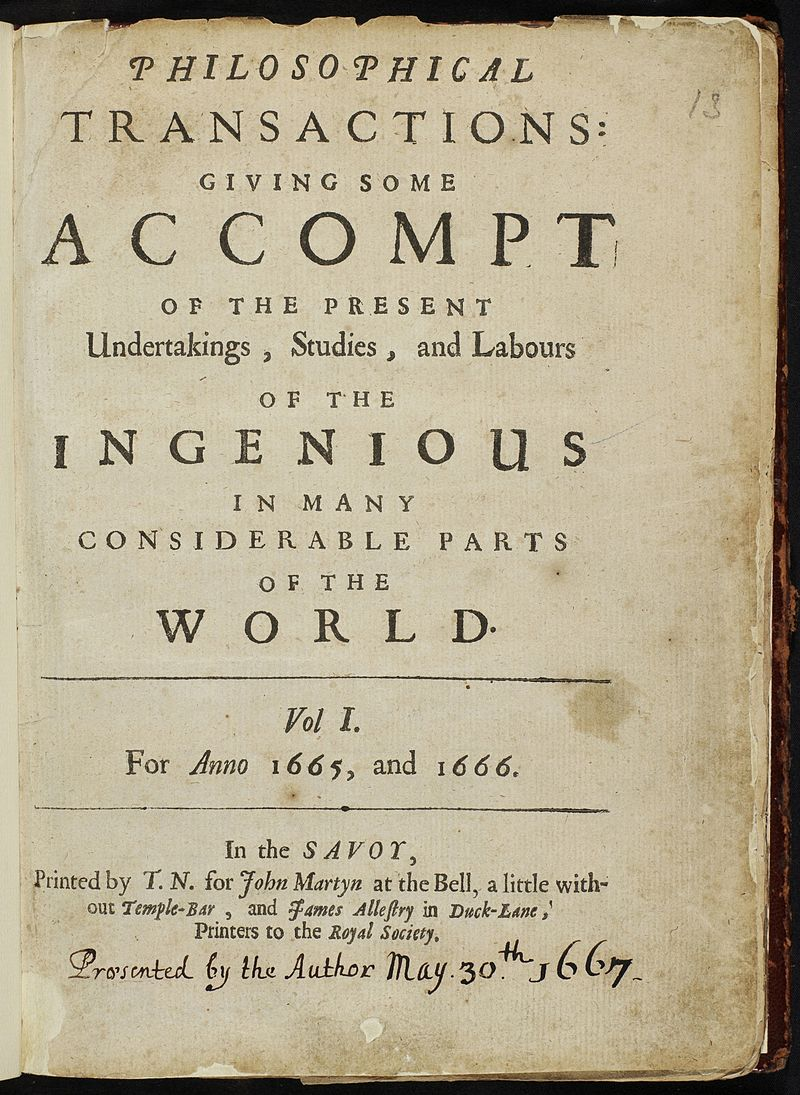
\includegraphics[scale=0.8]{figs/01/ptrslondon}
\end{figure}
\begin{itemize}
\item \small{\url{https://royalsocietypublishing.org/journal/rstl} }
\end{itemize}
\end{frame}

\section{Relevância da pesquisa científica}

%%
\begin{frame}
\begin{itemize}
\item A pesquisa é paga por pagadores de impostos, organizações e indivíduos
\item O final da linha: benefícios para a sociedade
\item Benefícios econômicos $\rightarrow$ oportunidades comerciais
\item Benefícios sociais $\rightarrow$ melhor qualidade de vida, sustentabilidade
\item Outros benefícios $\rightarrow$ extensão do conhecimento humano
\end{itemize}
\end{frame}

%%
\begin{frame}{O modelo linear da inovação}
\begin{figure}
\centering
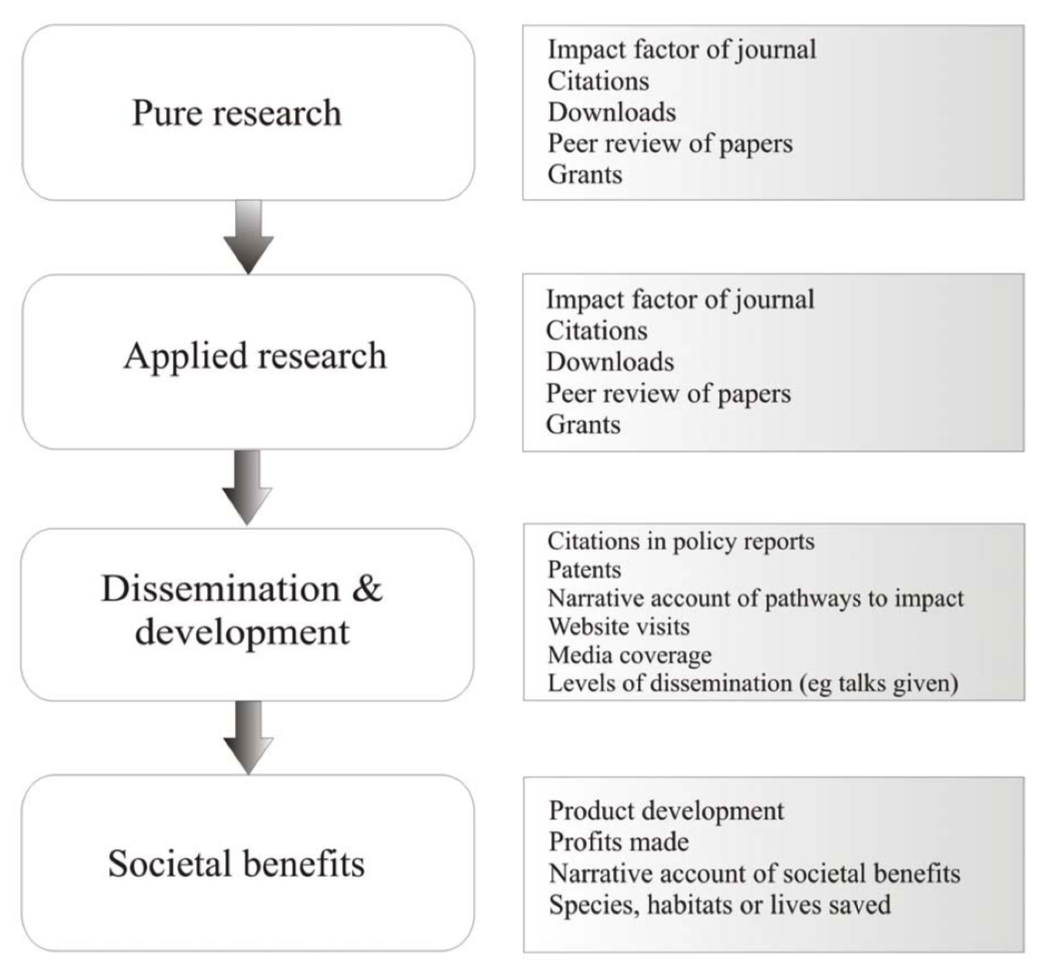
\includegraphics[scale=0.2]{figs/01/modelo-linear}
\caption{\small{Fonte: Sutherland, 2011 \textit{apud:} (Balconi, 2010).}}
\end{figure}
\end{frame}

\subsection*{Percepções da sociedade brasileira sobre C{\&}T}

%%
\begin{frame}{Otimismo sobre efeitos da C{\&}T}
\begin{figure}
\centering
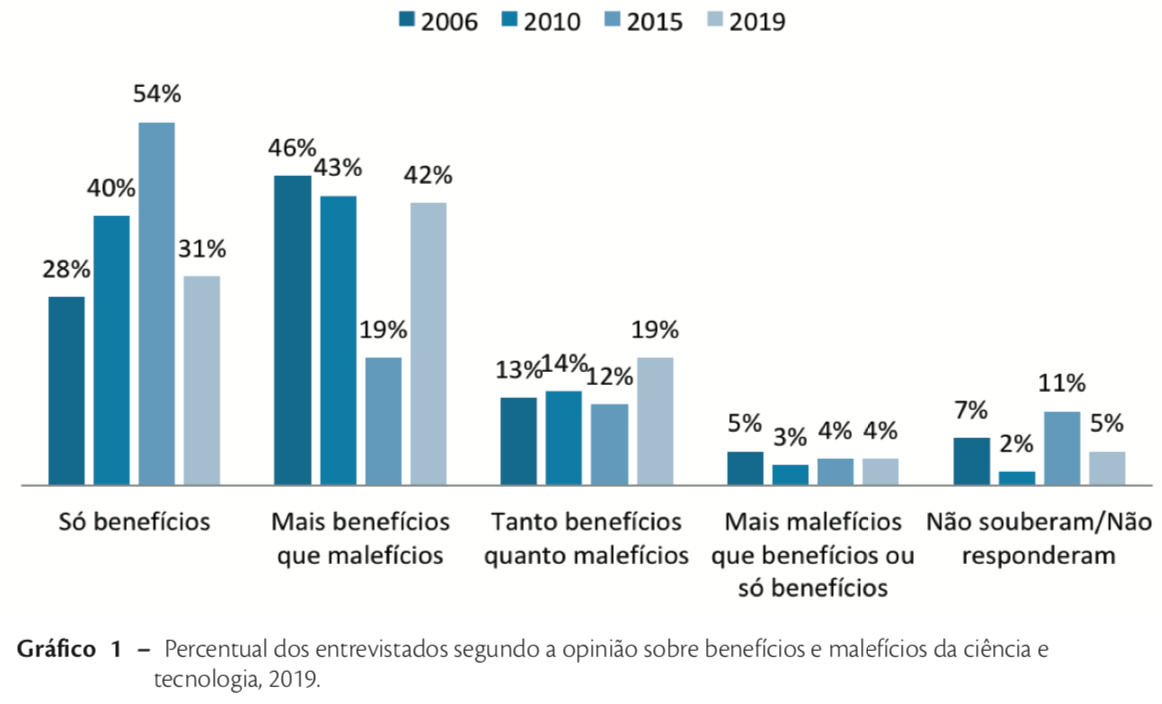
\includegraphics[scale=0.25]{figs/01/cet-otimismo}
\caption{Otimismo. Fonte: CGEE, 2019.}
\end{figure}
\end{frame}

%%
\begin{frame}{Imagem do cientista}
\begin{figure}
\centering
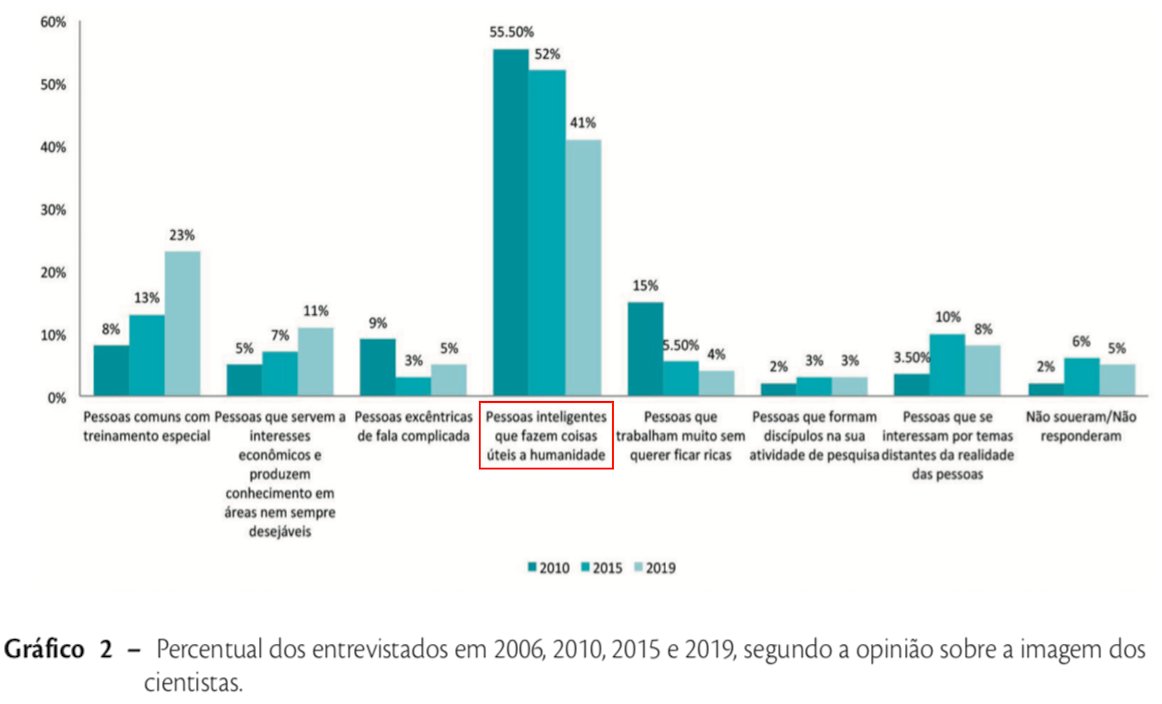
\includegraphics[scale=0.25]{figs/01/cet-imagem}
\caption{Imagem do cientista. Fonte: CGEE, 2019.}
\end{figure}
\end{frame}

%%
\begin{frame}{Índice de confiança}
\begin{figure}
\centering
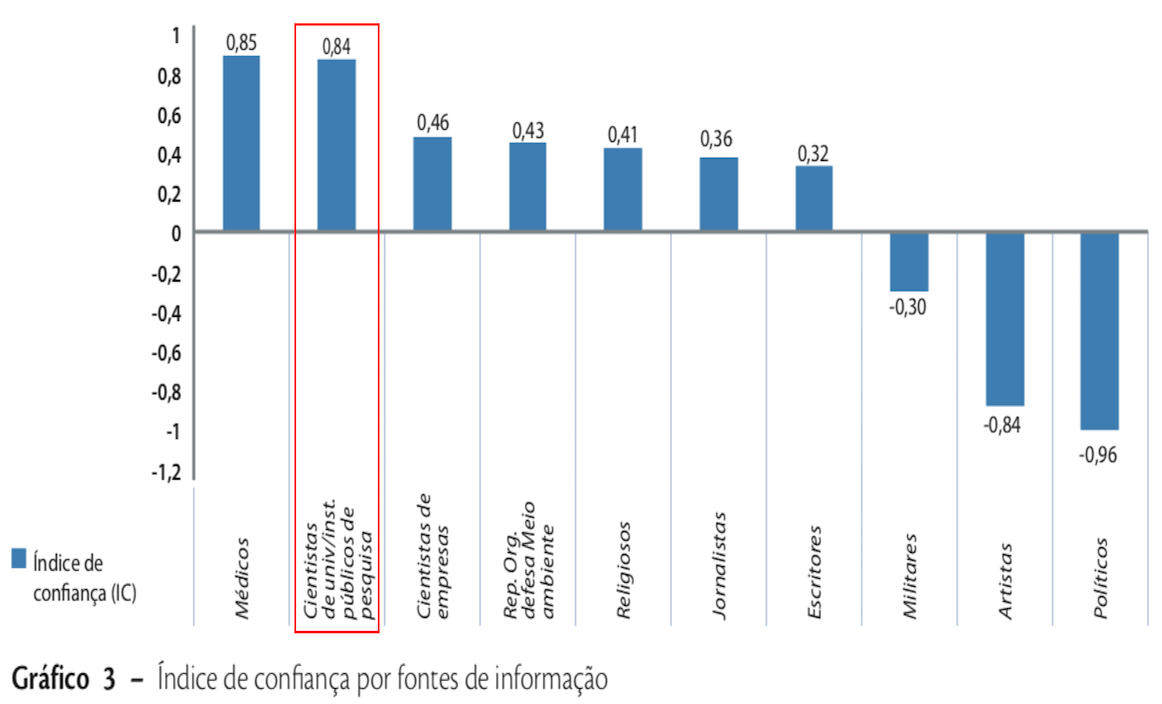
\includegraphics[scale=0.25]{figs/01/cet-ic}
\caption{Índice de confiança. Fonte: CGEE, 2019.}
\end{figure}
\end{frame}

\subsection*{O que é pesquisa?}

%%
\begin{frame}{O que é pesquisa?}
\begin{quotation}
Reunião de informações suficientes que respondem a uma questão que soluciona um problema. 
\end{quotation}
\begin{itemize}
\item Todos fazemos pesquisa, de certa forma: \\
>> Ex.: quando ocorreu o primeiro tremor de terra no Brasil? \\
>> Ex.: como a Google adquiriu seu atual valor de mercado?
\item Nem todos fazemos \textbf{pesquisa científica} \\
>> Ex.: o impacto da pesquisa científica no Brasil é melhor mensurado pelo número de artigos científicos publicados ou pelo número de patentes tecnológicas transferidas ao setor produtivo?
\end{itemize}
\end{frame}

\subsection*{Características do conhecimento científico}

%%
\begin{frame}
\begin{block}{Explicativo}
Busca compreender os fenômenos do mundo em multiescala, das ciências sociais à nanotecnologia, caracterizar elementos (variáveis) e detectar relações entre eles.
\end{block}
\end{frame}

%%
\begin{frame}
\begin{block}{Provisório}
Assume-se que todo conhecimento científico tem chance de ser negado no futuro; caso contrário, converte-se em um dogma.
\end{block}
\end{frame}

%%
\begin{frame}
\begin{block}{Lógico}
As conclusões científicas partem de pressupostos lógicos básicos, tais como dedução e indução para atingir conclusões. Analogias servem para especulações. Requer uma \textbf{base empírica}.
\end{block}
\end{frame}

%%
\begin{frame}
\begin{block}{Empírico}
O conhecimento requer uma base factual (empírica) para atender a expectativas teóricas (matemáticas ou não). A base empírica deve ser visível e reprodutível por outros. Se apenas você a detém ou enxerga, é uma crença, mesmo que seja verdadeira.
\end{block}
\end{frame}


\subsection*{Por que escrever a pesquisa?}

%%
\begin{frame}
\begin{itemize}
\item Um dia alguém poderá fazer a mesma pergunta de hoje
\item A pesquisa que você faz poderá responder tal pergunta
\item Pesquisas publicadas (sérias e confiáveis) evitam que sejamos aprisionados em idéias próprias equivocadas ou em experiências solitárias inférteis.
\end{itemize}
\end{frame}

%%
\begin{frame}
\begin{itemize}
\item Publicações estimulam o ``ceticismo amigável''
\item Se isto vale, até quando? (São 9 planetas mesmo?) 
\item O ponto central é formar opinião, desenvolver o pensamento crítico e combater o ``charlatanismo'' científico (Tomar café demais pode matar... Cafeína é bom para o sangue...)
\end{itemize}
\end{frame}

%%
\begin{frame}{O que se ganha escrevendo?}
\begin{block}{Escreva para lembrar-se}
Pessoas sortudas retêm informação sem necessidade de registros. Nem todos temos esse dom. Aliás... qual era a pressão aplicada no experimento A.29 do dia 01/05/2019? Logo, você ganha \textbf{apenas uma (crucial) lembrança}. 
\end{block}
\end{frame}


%%
\begin{frame}{O que se ganha escrevendo?}
\begin{block}{Escreva para entender}
Ao organizar e reorganizar seus dados de pesquisa, você descobre novas conexões, contrastes, complicações e implicações. Então, você consegue \textbf{ampliar padrões de significado}. $(0.5a + 0.5b) = \frac{a+b}{2}$, mas a segunda forma é mais ``límpida''...
\end{block}
\end{frame}


%%
\begin{frame}{O que se ganha escrevendo?}
\begin{block}{Escreva para ganhar perspectiva}
Os pensamentos na sua mente são menos claros do que quando postos no papel. Lá dentro da caixa, estão no escuro e no calor. No papel, eles são claros como a luz do dia. E é aí que você se depara com a célebre frase: ``não era bem isso que eu queria dizer... '' \texttt{:]}. Portanto, você ganha \textbf{coerência, clareza e organização de pensamento}. 
\end{block}
\end{frame}


\subsection*{Por que reportar uma pesquisa formalmente?}

%%
\begin{frame}{Perguntas legítimas}
\begin{itemize}
\item Por que devo me submeter a padrões restritos? 
\item Por que devo obedecer o estilo imposto pela comunidade?
\item Por que devo adotar uma linguagem técnica? 
\end{itemize}
\end{frame}


%%
\begin{frame}{Respostas legítimas}
\begin{itemize}
\item Porque você testa a força ou fraqueza de seus argumentos.
\item Porque você confronta suas idéias com os padrões e valores dos outros.
\item Porque escrever para outros exigirá seu esforço pessoal.
\end{itemize}
\end{frame}


%%
\begin{frame}{Seu leitor vai querer saber...}
\begin{itemize}
\item Como você avaliou a evidência A?
\item Por que você acha que X é mais relevante do que Y?
\item Como você responde o fato de Z não ser z, mas ambas serem ``zê''? 
\end{itemize}
\end{frame}

\section{Panorama da produção científica brasileira}

%%
\begin{frame}{Número de artigos: tabela}
\begin{figure}
\centering
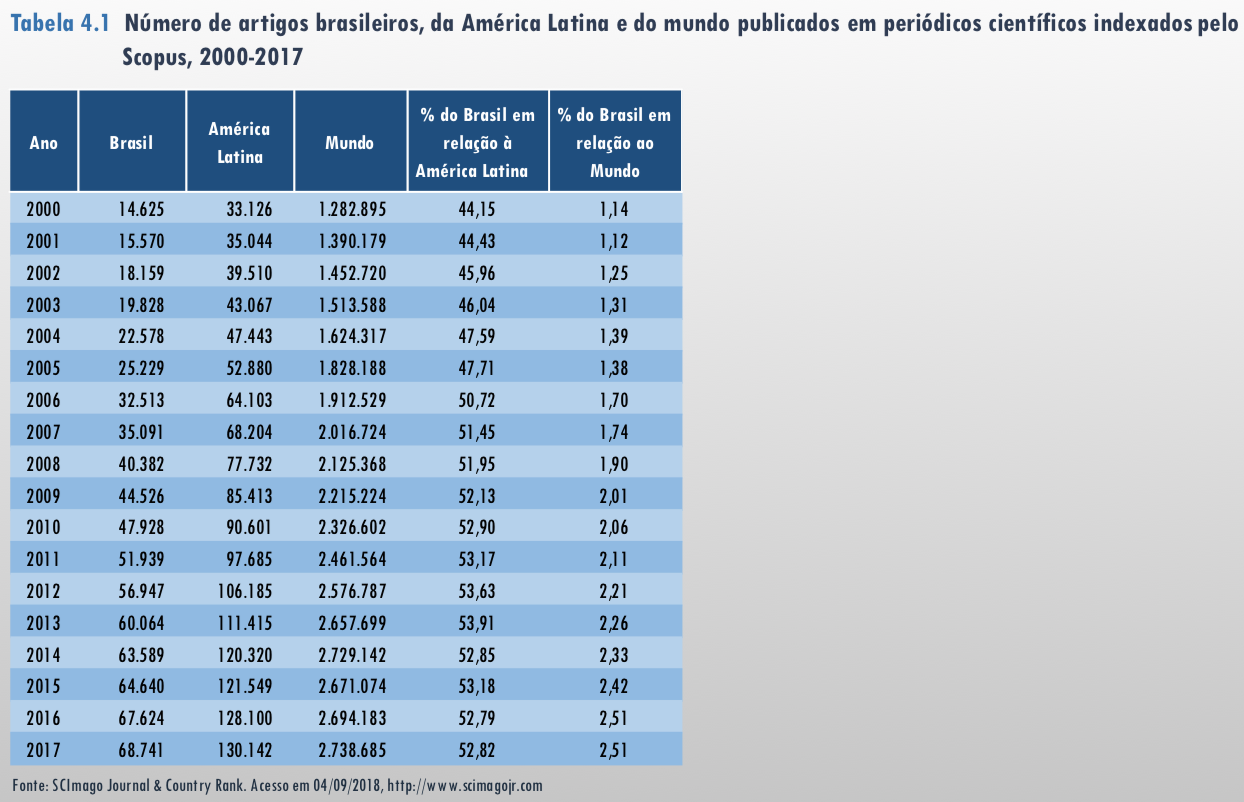
\includegraphics[scale=0.25]{figs/01/panorama-artigos-tabela}
\caption{Artigos. Fonte: COIND/MCTIC, 2018.}
\end{figure}
\end{frame}

%%
\begin{frame}{Número de artigos: gráfico}
\begin{figure}
\centering
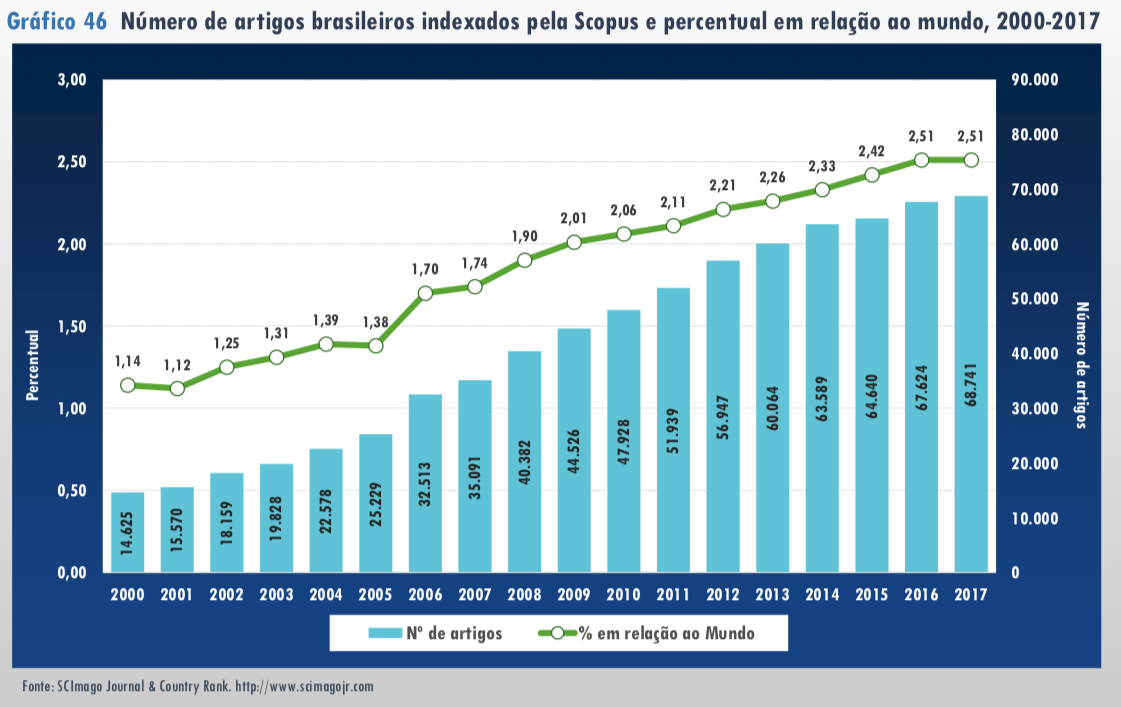
\includegraphics[scale=0.25]{figs/01/panorama-artigos}
\caption{Artigos - gráfico. Fonte: COIND/MCTIC, 2018.}
\end{figure}
\end{frame}

%%
\begin{frame}{Número de citações: tabela}
\begin{figure}
\centering
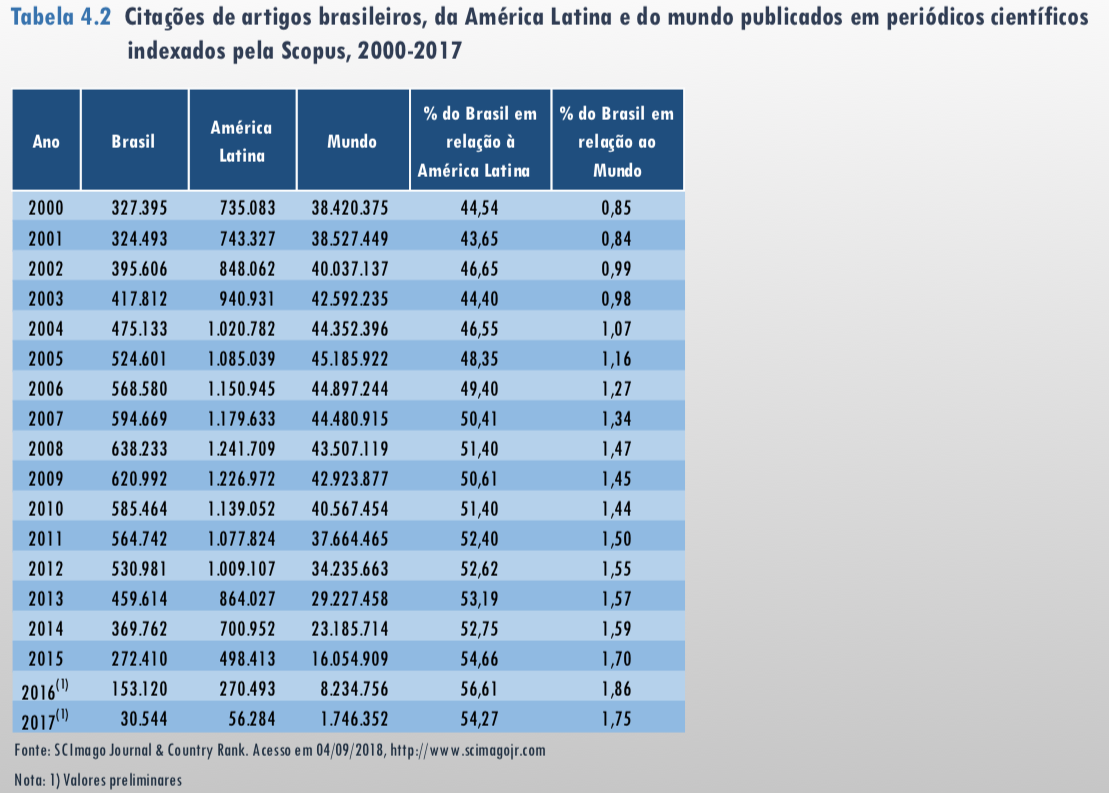
\includegraphics[scale=0.25]{figs/01/panorama-citacoes-tabela}
\caption{Citações. Fonte: COIND/MCTIC, 2018.}
\end{figure}
\end{frame}

%%
\begin{frame}{Número de citações: gráfico}
\begin{figure}
\centering
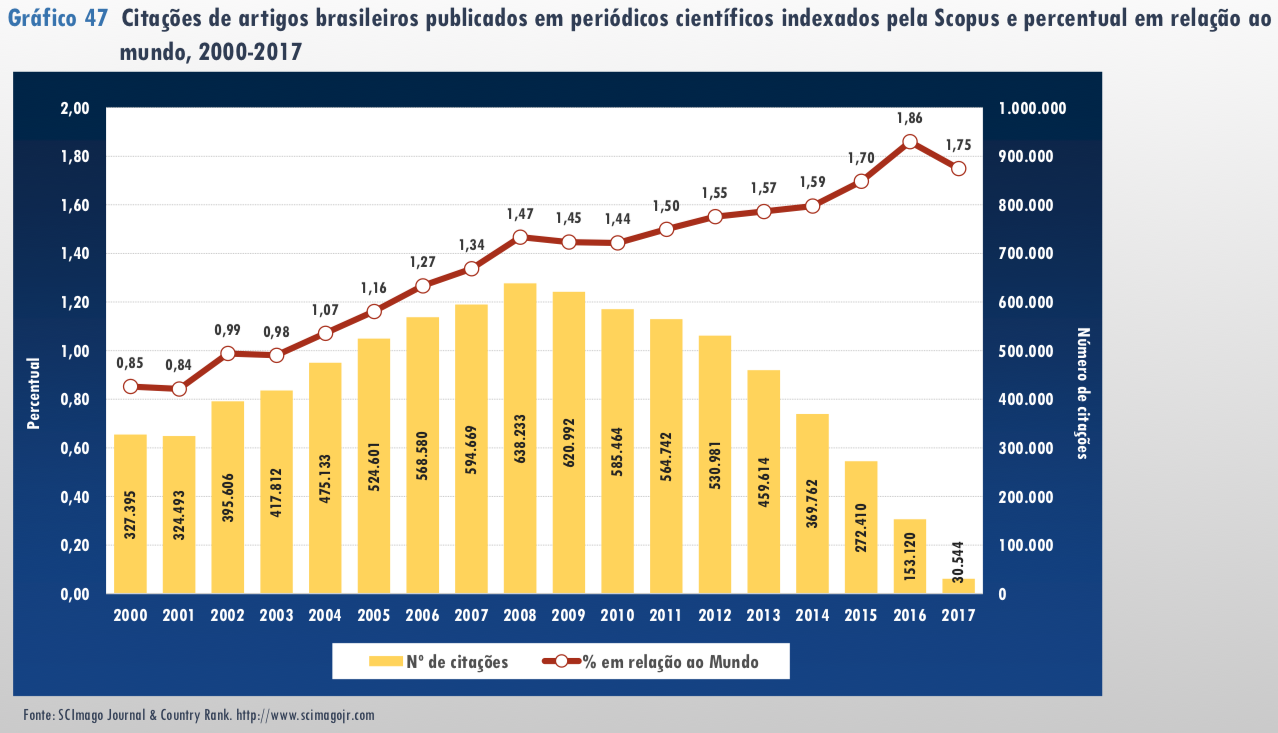
\includegraphics[scale=0.25]{figs/01/panorama-citacoes}
\caption{Citações - gráfico. Fonte: COIND/MCTIC, 2018.}
\end{figure}
\end{frame}

%%
\begin{frame}{Produtividade}
\begin{figure}
\centering
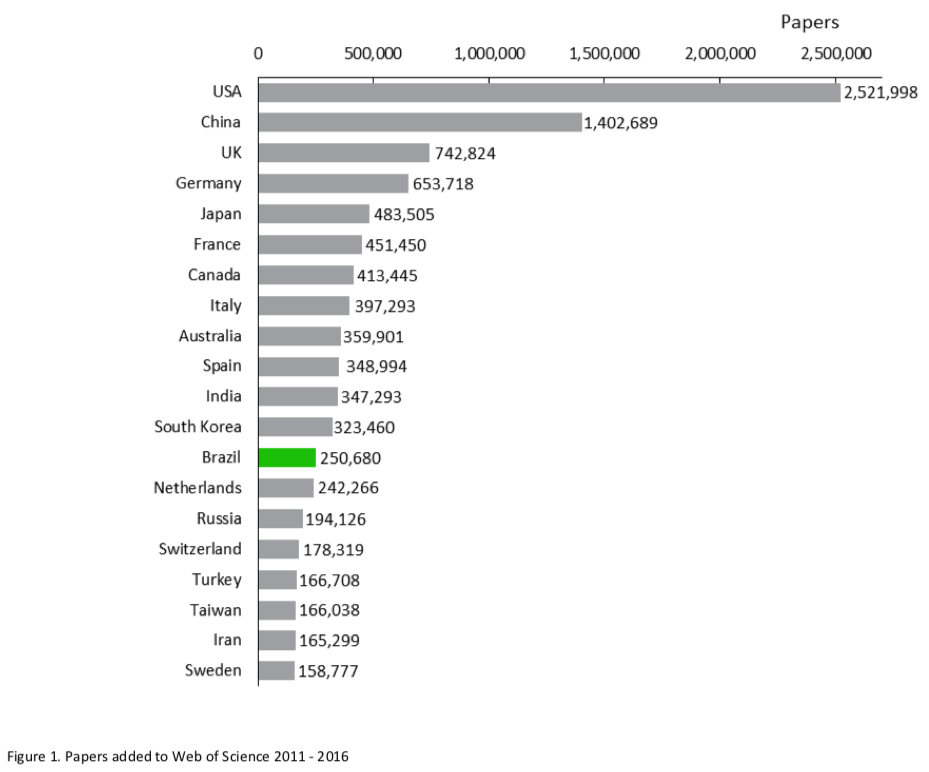
\includegraphics[scale=0.25]{figs/01/panorama-produtividade}
\caption{Produtividade. Fonte: Clarivate Analytics, 2017.}
\end{figure}
\end{frame}

%%
\begin{frame}{Impacto por citações}
\begin{figure}
\centering
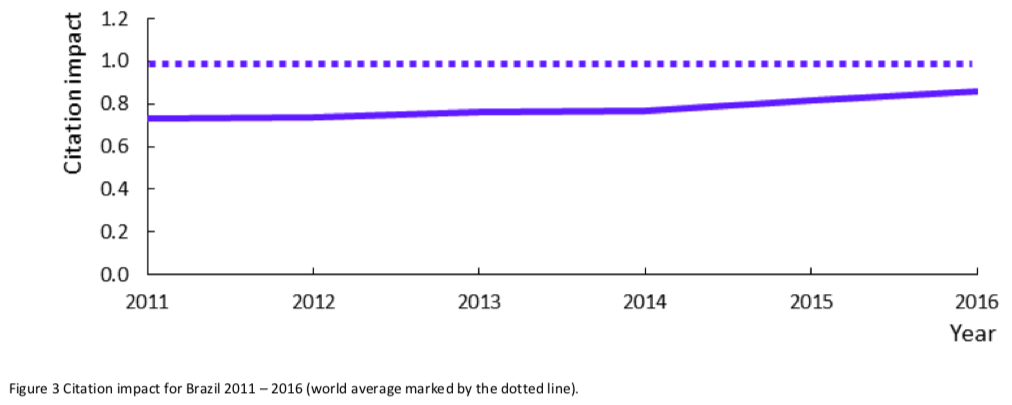
\includegraphics[scale=0.3]{figs/01/panorama-impacto-citacao}
\caption{Impacto por citações. Fonte: Clarivate Analytics, 2017.}
\end{figure}
\end{frame}

%%
\begin{frame}{Colaboração internacional - Top 20}
\begin{figure}
\centering
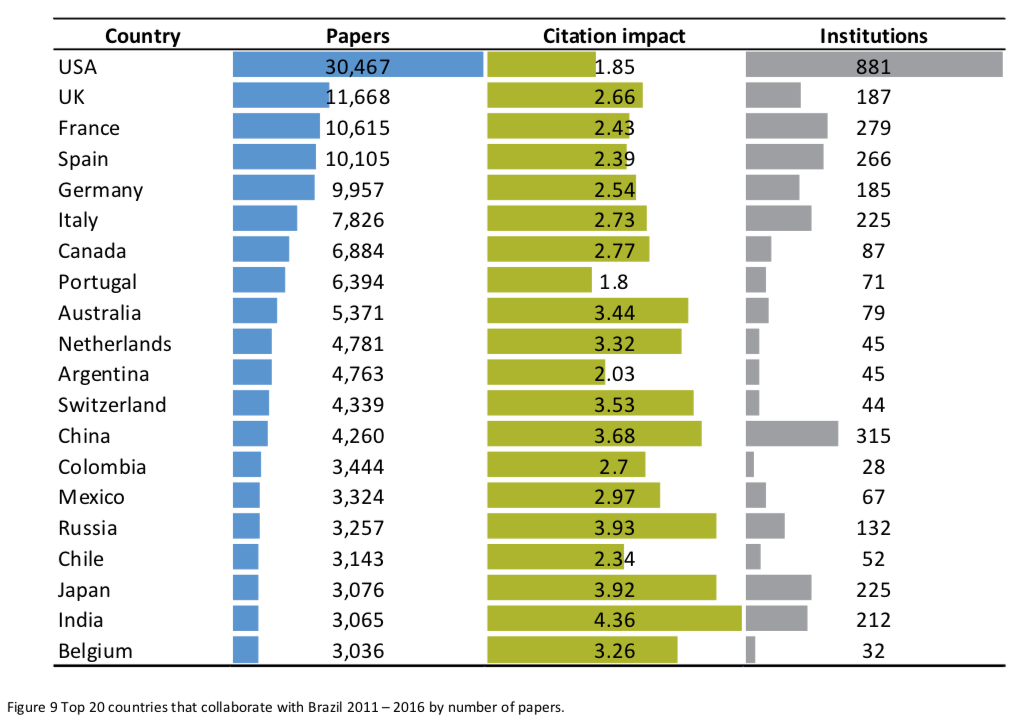
\includegraphics[scale=0.25]{figs/01/panorama-top20}
\caption{\scriptsize{Colaboração internacional. Fonte: Clarivate Analytics, 2017.}}
\end{figure}
\end{frame}

%%
\begin{frame}{Colaboração internacional com empresas - Top 20}
\begin{figure}
\centering
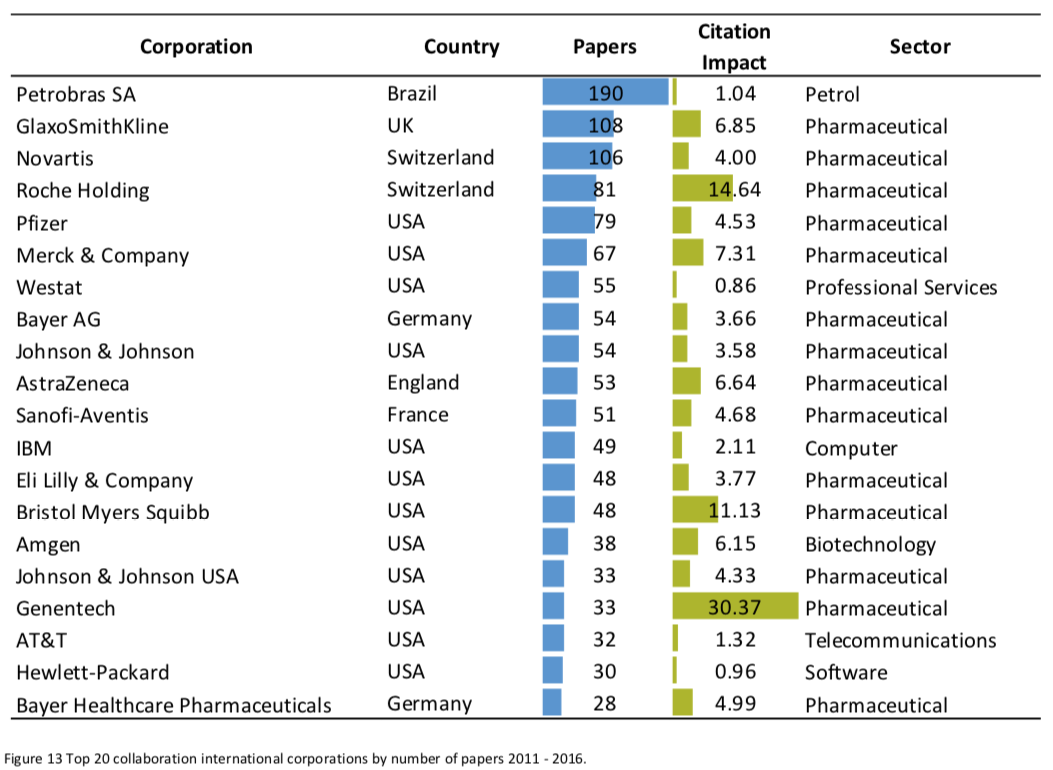
\includegraphics[scale=0.25]{figs/01/panorama-top20-papers}
\caption{\scriptsize{Colaboração internacional com empresas. Fonte: Clarivate Analytics, 2017.}}
\end{figure}
\end{frame}

%%
\begin{frame}{Comparação com outros países}
\begin{figure}
\centering
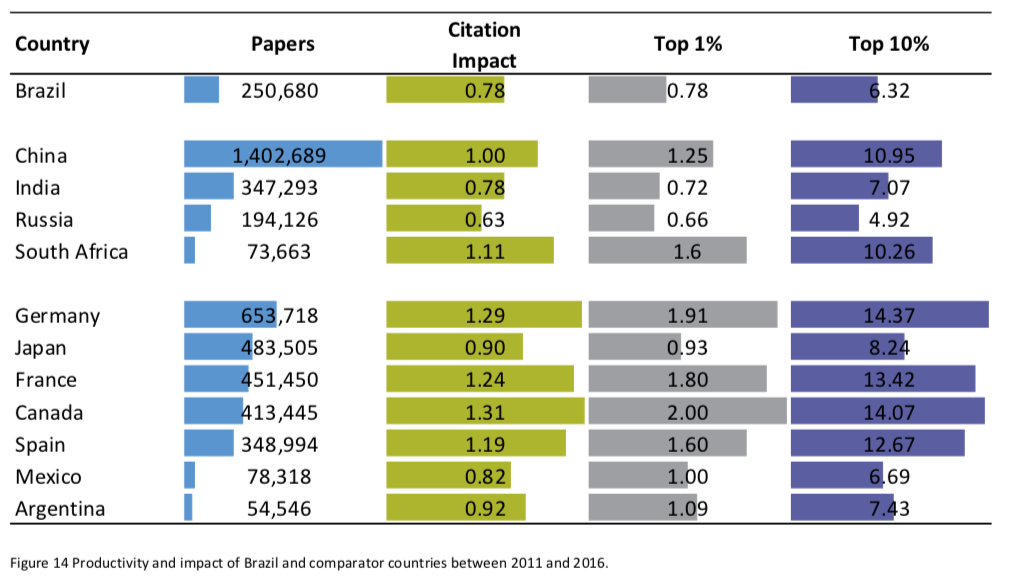
\includegraphics[scale=0.25]{figs/01/panorama-prod-paises}
\caption{Comparação com outros países. Fonte: Clarivate Analytics, 2017.}
\end{figure}
\end{frame}


%%
\begin{frame}{Efeito da colaboração internacional sobre produtividade}
\begin{figure}
\centering
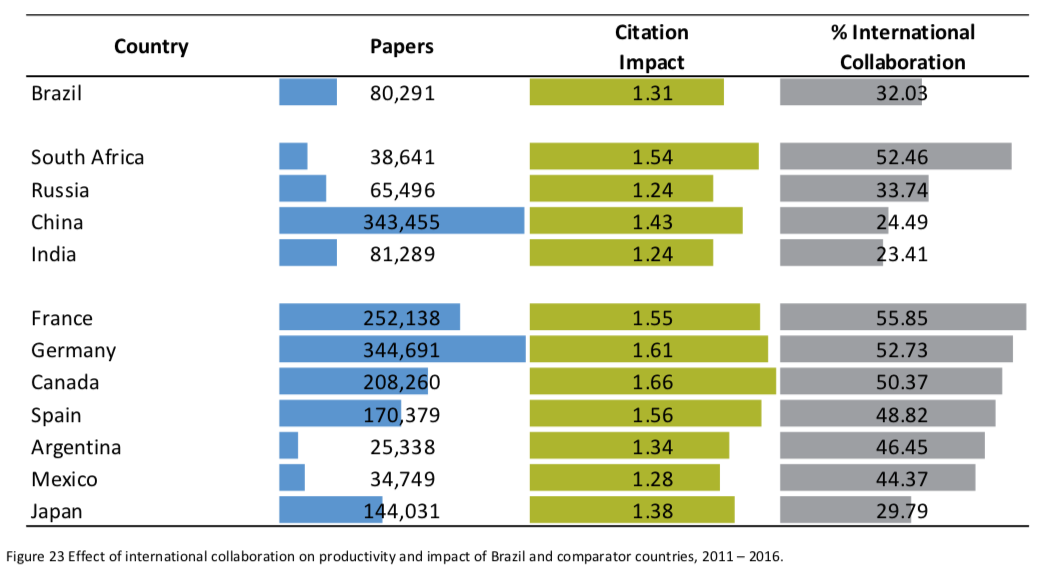
\includegraphics[scale=0.25]{figs/01/panorama-colaboracao}
\caption{Efeito da colaboração internacional sobre produtividade. Fonte: Clarivate Analytics, 2017.}
\end{figure}
\end{frame}


%%
\begin{frame}{Artigos brasileiros por área - Top 30}
\begin{figure}
\centering
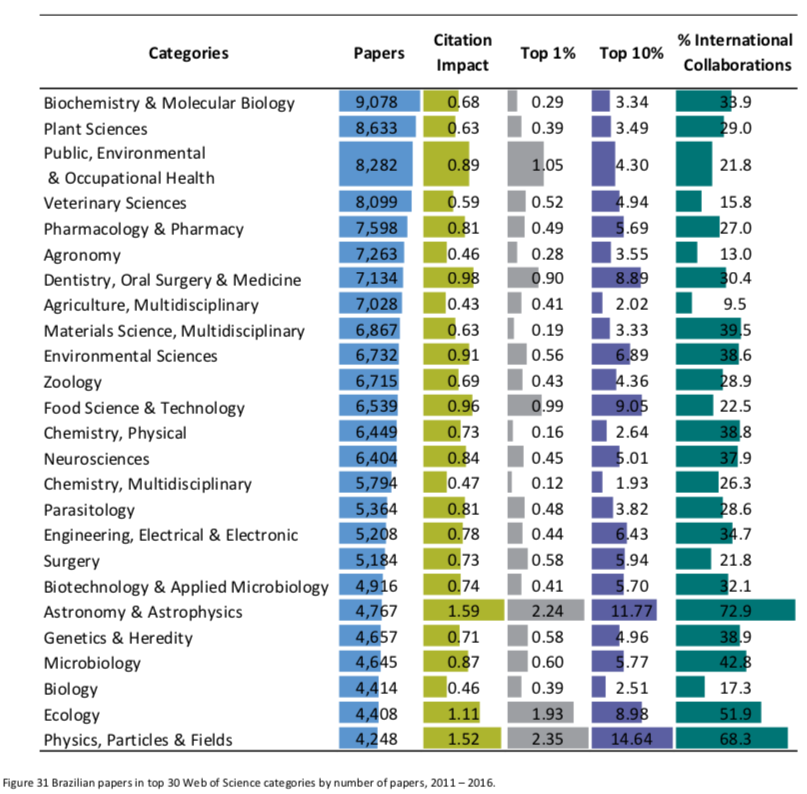
\includegraphics[scale=0.25]{figs/01/panorama-top30}
\caption{\scriptsize{Artigos brasileiros por área - Top 30. Fonte: Clarivate Analytics, 2017.}}
\end{figure}
\end{frame}

%%
\begin{frame}{Desempenho por estados da federação}
\begin{figure}
\centering
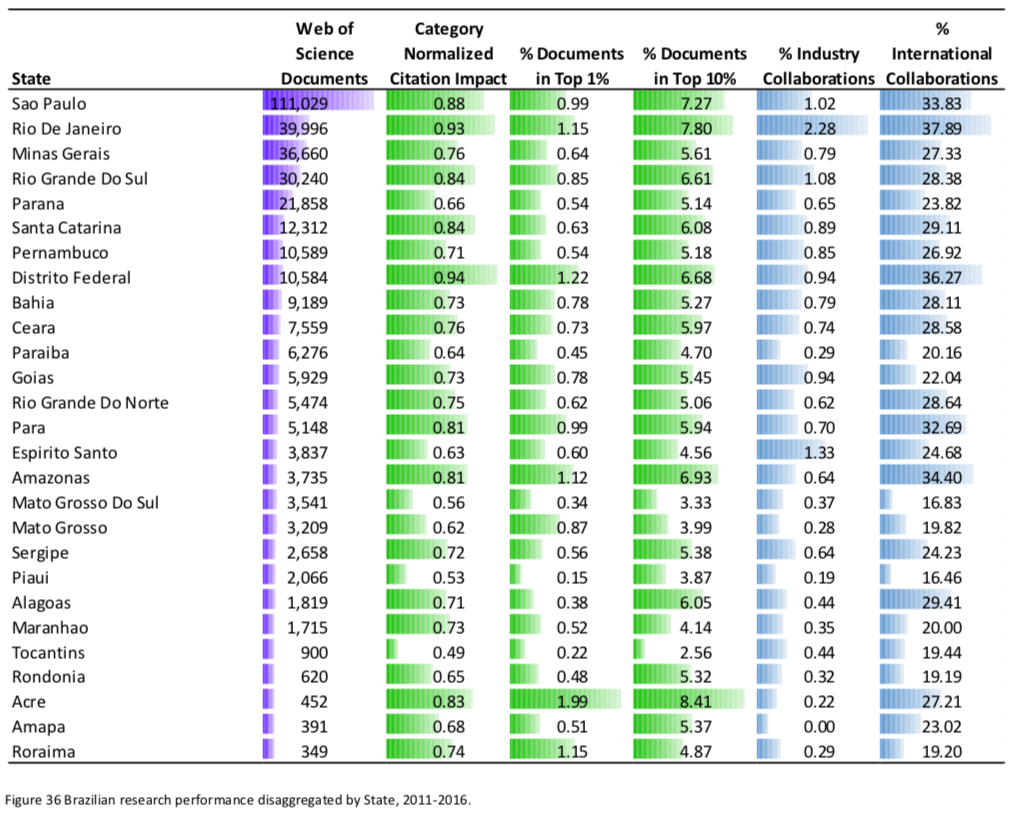
\includegraphics[scale=0.2]{figs/01/panorama-estados}
\caption{\scriptsize{Desempenho por estados. Fonte: Clarivate Analytics, 2017.}}
\end{figure}
\end{frame}

%%
\begin{frame}{Universidades com melhor desempenho}
\begin{figure}
\centering
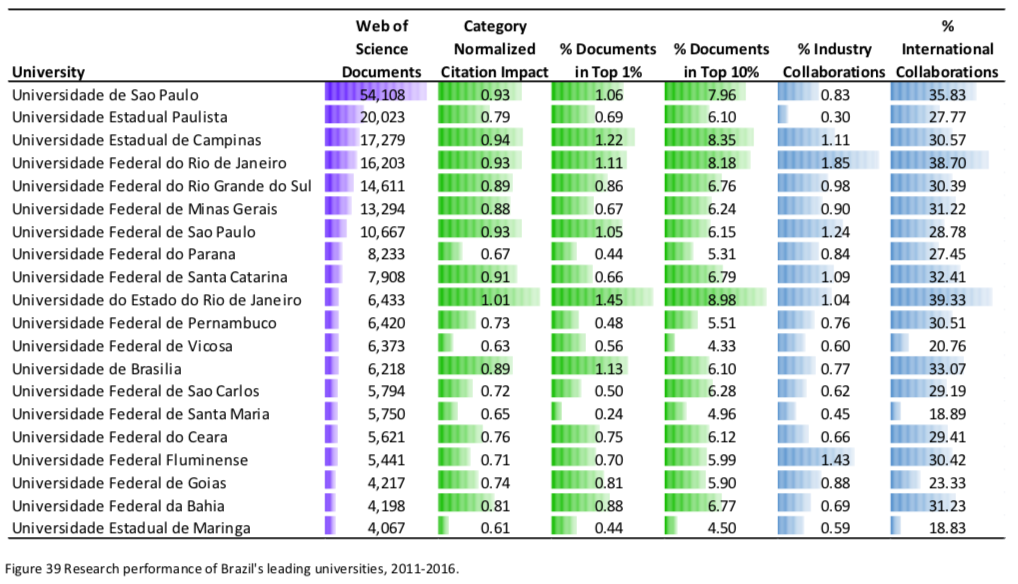
\includegraphics[scale=0.27]{figs/01/panorama-univs}
\caption{Universidades com melhor desempenho. Fonte: Clarivate Analytics, 2017.}
\end{figure}
\end{frame}

\section{Metodologia científica na pós-graduação} 

\subsection*{Atividade científica}

%%
\begin{frame}{O mínimo a saber...}
\begin{itemize}
\item Legislação básica: pareceres 977/65 e 77/69 CFE.
\item Cabe à CAPES avaliar e acompanhar a pós-graduação no Brasil 
\item Plano Nacional de Pós-Graduação (PNPG 2011 - 2020)
\end{itemize}
\end{frame}

\subsection*{Perfil da produção científica}

%%
\begin{frame}{Caractarísticas qualitativas}
O trabalho de pesquisa é: 

\begin{itemize}
\item \textit{pessoal}: é um comprometimento; fará parte da sua vida
\item \textit{autônomo}: é fruto de esforço próprio; seu orientador será um mentor 
\item \textit{criativo}: é mais do que aprender; não só técnica e método; misto de paixão e razão
\item \textit{rigoroso}: é profissional, ético e correto; não cabe senso comum nem mediocridade
\end{itemize}
\end{frame}

\subsection*{Trabalhos acadêmicos}

%%
\begin{frame}{A dissertação de mestrado}
\begin{itemize}
\item comunica resultados de uma pesquisa e reflexão
\item é elaborada com diretrizes metodológicas, técnicas e lógicas
\item difere da tese de doutorado no nível de originalidade
\item é um trabalho de amadurecimento na caminhada científica
\end{itemize}
\end{frame}

%%
\begin{frame}{A tese de doutorado}
\begin{itemize}
\item é o tipo mais representativo do trabalho científico monográfico
\item aborda um único tema suficientemente original, específico, delimitado e restrito
\item soluciona um problema com sólidas argumentações
\item empurra a fronteira do conhecimento com uma contribuição nova
\end{itemize}
\end{frame}

%%
\begin{frame}{Natureza da dissertação ou tese}
\begin{itemize}
\item \textit{caráter monográfico}: ater-se ao substancial da pesquisa; evitar historicidades amplas, repetições ou ``reinventar a roda''
\item \textit{coerência}: o texto deve possuir coerência lógico-estrutural do raciocínio (nível 1); coerência de premissas, referencial teórico, método (nível 2)
\end{itemize}
\end{frame}

\subsection*{Eventos}

%%
\begin{frame}
\begin{block}{Congresso}
Reunião para discussão e debate de idéias, promovido em geral por especialistas e interessados na área.
\end{block}

\begin{block}{Conferência}
Similar ao congresso, mas é mais amplo, visto que reúne muito mais (senão todas) as entidades de uma determinada área.
\end{block}
\end{frame}

%%
\begin{frame}
\begin{block}{Palestra}
É uma ``conferência menos solene'', feita por um expositor único, podendo ser isolada ou não.
\end{block}

\begin{block}{Encontro}
Evento de menor porte que o Congresso e mais abrangente do que uma simples reunião. 
\end{block}
\end{frame}

%%
\begin{frame}
\begin{block}{Jornada}
Encontro que faz referência a um certo tempo, em termos de dias. Similar a Encontro ou Congresso.
\end{block}

\begin{block}{Simpósio}
Reunião destinada apenas a especialistas para discussão de tema previamente determinado.
\end{block}
\end{frame}

%%
\begin{frame}
\begin{block}{Seminário}
Reunião mais restrita como grupo de estudos em que se discute um tema com a contribuição de todos os participantes.
\end{block}

\begin{block}{Sessões de Comunicação}
Ocorrem em geral em eventos de grande porte, na forma de \textit{Keynote Speakers}.
\end{block}
\end{frame}

%%
\begin{frame}
\begin{block}{Mesa-Redonda}
Apresentação de pontos de vista diferentes sobre uma mesma questão.
\end{block}

\begin{block}{Painel}
Apresentação de trabalhos sobre um mesmo tema, abordado sob pontos de vista diferentes.
\end{block}
\end{frame}

%%
\begin{frame}
\begin{block}{Oficinas (\textit{Workshops})}
Reuniões restritas em número de participantes para apresentação de trabalhos, experiências, em geral com caráter prático.
\end{block}

\begin{block}{Apresentação de pôsteres}
São as chamadas \textit{Poster Sessions}, onde se apresentam trabalhos por meio de pôsteres.
\end{block}
\end{frame}


\subsection*{O artigo como motor de pesquisa}

%%
\begin{frame}{Principal ``produto'' da escrita científica}
\begin{figure}
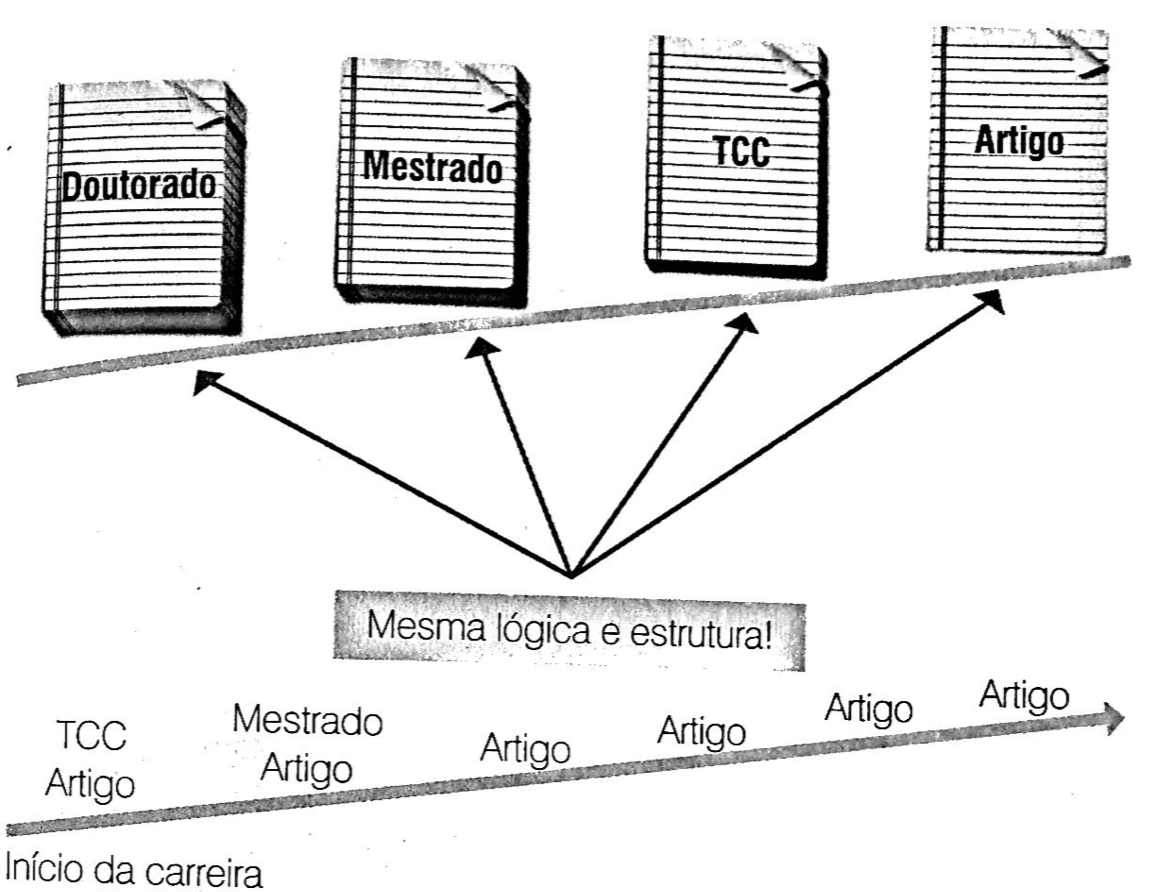
\includegraphics[scale=0.4]{figs/01/ilustracao-artigo}
\caption{Fonte: Volpato}
\end{figure}
\end{frame}

\begin{frame}{Características}
\begin{itemize}
\item Destinado especificamente à publicação em revistas e periódicos
\item Registra e divulga pesquisa sobre temas não devidademente explorados
\item Esclarece questões em discussão no meio científico
\item Contém objetivos, fundamentação teórica, metodologia, análise de dados e/ou discussão, conclusões e referências bibliográficas
\item É formatado de acordo com normas específicas de um publicador
\end{itemize}
\end{frame}

\section{Suplementos}

\begin{frame}{Órgãos federais para CT{\&I}}
\begin{itemize}
\item MCTIC: \url{http://mctic.gov.br}
\item CNPq: \url{http://cnpq.br}
\item CAPES: \url{http://cnpq.br}
\end{itemize}
\end{frame}

%%
\begin{frame}{Recursos}
\begin{itemize}
\item QUADRIENAL/CAPES: \url{http://avaliacaoquadrienal.capes.gov.br/documentos-de-area}
\item SDI/CAPES: \url{http://sdi.capes.gov.br}
\item PNPG/CAPES: \url{https://www.capes.gov.br/plano-nacional-de-pos-graduacao}
\item Sucupira/CAPES: \url{https://sucupira.capes.gov.br/sucupira/}
\item IBICT: \url{http://www.ibict.br}
\end{itemize}
\end{frame}


%%
\begin{frame}{Sugestão de leitura...}
\url{https://www.scribendi.com/advice/publish_or_perish.en.html}
\end{frame}

%% === REFS
\begin{frame}[allowframebreaks]
\frametitle{Referências}
\begin{thebibliography}{9}
\setbeamertemplate{bibliography item}[book]
%
\bibitem{day1993} Day, R. A., \textit{How to write and publish scientific papers}, Cambridge University Press, 1995.
%
\bibitem{booth2003} Booth, W. et al., \textit{The craft of research}, University of Chicago Press, 2003.
%
\bibitem{sutherland2011} Sutherland, W.J., et al., \textit{Quantifying the impact and relevance of scientific research}. PLoS One, 6(11), 2011.

\bibitem{cgee2019} Centro de Gestão e Estudos Estratégicos - CGEE, \textit{Percepção Pública da C{\&}T no Brasil - 2019}. Resumo Executivo. Brasília, DF: 2019, 24p.

\bibitem{mctic2018} Coordenação de Indicadores e Informação - COIND, \textit{Indicadores Nacionais de Ciência, Tecnologia e Inovação - 2018}, Brasília, MCTIC, 2018.

\bibitem{clarivate2018} Cross, D.; Thomson, S.; Sinclair, A. \textit{Research in Brazil: A report for CAPES by Clarivate Analytics}. Clarivate Analytics, 2018.

\bibitem{volpato2017}Volpato, G.L. \textit{Método Lógico para Redação Científica}. 2a. ed., Best Writing, 2017.

\bibitem{severino}Severino, A.J. \textit{Metodologia do Trabalho Científico}, 24a. ed., Cortez Editora, 2017.


\end{thebibliography}
\end{frame}